\chapter{An Implementational Framework \\ for the DG-PEM} \label{ch:implementation}
%
The implementation of a given partitioned element method must address two primary challenges: the subdivision of an element into cells, and the solution of shape function boundary value problems by way of the chosen PEM formulation. The first of these two tasks may be accomplished in various ways, some of them more complicated than others. Herein we propose a relatively simple element partitioning algorithm which necessitates that the elements and their faces be simply connected, and star-convex.

The present implementational framework is directed at obtaining DG-PEM approximations to harmonic shape functions on arbitrary polytopes -- i.e. solving (\ref{eq:dg_poisson}) on an appropriately defined partition of the element.

\section{Arbitrary Polytopal Meshes}

	Traditional finite element methods typically only permit the elements to take the form of certain canonical shapes with fixed topology (most commonly tetrahedra or hexahedra). This yields several benefits with regard to the data and storage requirements necessary to represent a given element in a computational setting. Frequently, it suffices to describe the geometry of a canonical shape (such as a hexahedron) by providing a list of the element's nodal coordinates, along with an ordered sequence of the element's node IDs which fully determines its resulting topology (and its faces, edges) according to some conventional node numbering scheme (refer to Figure \ref{fig:canonical_orderings} as a representative example.)
	\begin{figure} [!ht]
		\centering
		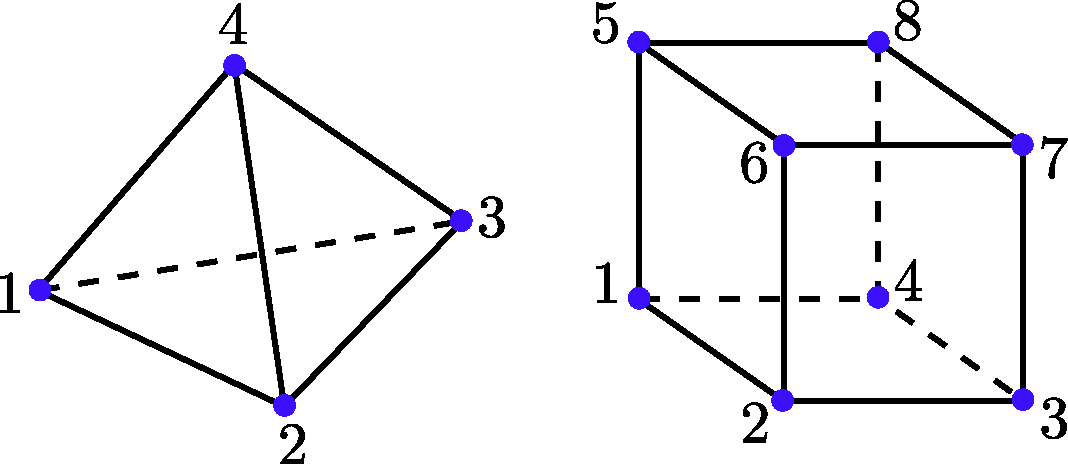
\includegraphics[width = 4.0in]{figures/canonical_orderings.pdf}
		\caption{Canonical node numbering schemes for a linear tetrahedral element (left) and a linear hexahedral element (right).}
		\label{fig:canonical_orderings}
	\end{figure}
	
	Polytopal elements with arbitrary topology (with a variable number of nodes, edges, and faces) cannot be represented in this fashion. As a consequence, more descriptive data structures are necessary to fully determine a given element's nodal connectivity. A particular scheme to represent an arbitrary polyhedron in a finite element mesh is described in the following section.

\subsection*{Geometric Data Structures for Arbitrary Polytopes}

	There are multiple ways in which the geometry of a given polyhedral element $\Omega$ may be represented within a finite element code. Ideally, however, the chosen data structure should be made as compact as possible, for the purposes of minimizing the storage requirements of a single element. This section describes a few basic data structures for storing arbitrary polgonal and polyhedral shapes within an unstructured finite element mesh.
	
	It is assumed that the mesh geometry for a finite element discretiztion of the model problem described in chapter \ref{ch:solid_mechanics} may be generically characterized by:
	\begin{itemize}
		\item A list of all nodal coordinates $\left\{ \mathbf{X}_a \right\}_{a=1}^{N_V}$. The sub-index $a \in 1, \ldots, N_V$ induces a \textit{global node ID} ascribed to each node.
		\item A list of all elements $\left\{ \Omega_{e} \right\}_{e = 1}^{N_\Omega}$ where $\Omega_{e} \subset \mathcal{B}_0$. The sub-index $e \in 1, \ldots, N_\Omega$ induces an associated \textit{element ID}.
		\item A list of all faces $\left\{ F_{b} \right\}_{b = 1}^{N_F}$ where $F_{b} \subset \Gamma^N_0$ to which traction boundary conditions are assigned. Likewise, the sub-index $b \in 1, \ldots, N_F$ induces a \textit{boundary face ID}.
	\end{itemize}
	
	In a finite element mesh consisting of arbitrary polyhedral elements, it is suggested that each element $\Omega_e$ be represented by the following data:
	\begin{itemize}
		\item A list of the global node IDs $\left\{ a_i \right\}_{i=1}^{N^e_V}$ comprising the set of nodes belonging to $\Omega_e$. The sub-index $i \in 1, \ldots, N^e_V$ induces a \textit{local node ID}, particular to the element $\Omega_e$.
		\item A list of the polygonal faces $\left\{ F_{j} \right\}_{j=1}^{N^e_F}$ which belong to $\partial \Omega_e$; each polygonal face $F_j$ is in turn represented by a cycle of local node IDs denoted $\left\{ n_i \right\}_{i=1}^{N^j_V}$, which further determine each face's outward orientation with respect to the element $\Omega_e$.
	\end{itemize}
	An illustration of this collection of data for a given polyhedron $\Omega_e$ is provided in Figure \ref{fig:polyhedron_data}.
	\begin{figure} [!ht]
		\centering
		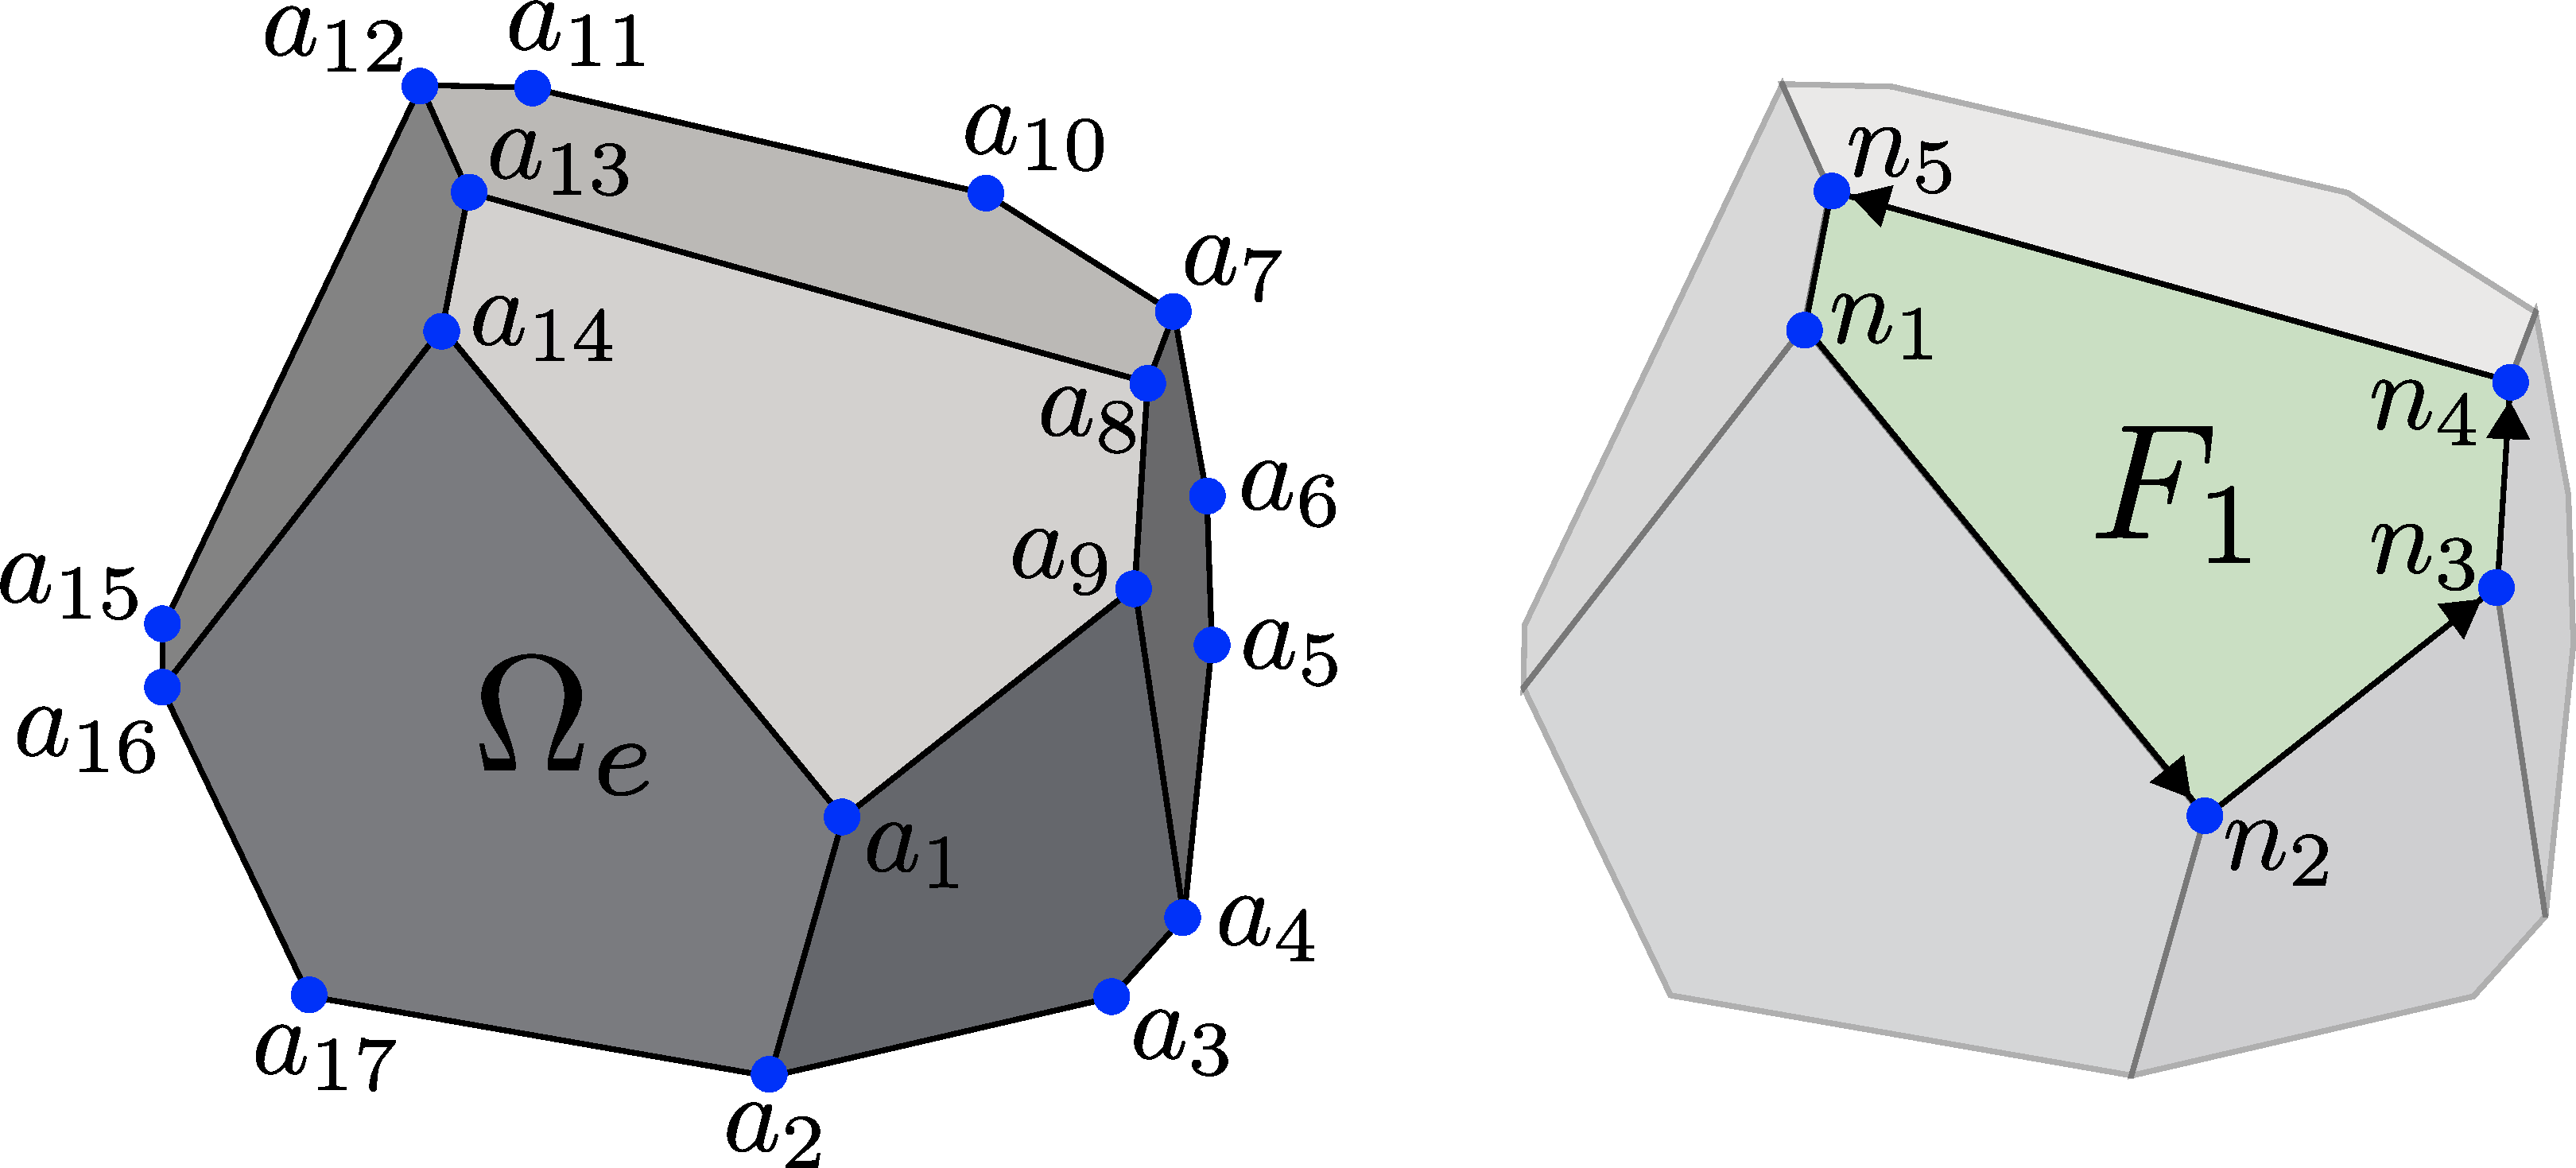
\includegraphics[width = 6.0in]{figures/polyhedron_data.pdf}
		\caption{Illustration of the data necessary to describe an arbitrary polyhedral element $\Omega_e$. The local node ID ordering for the face $F_1$ shown would be $\left\{ n_i \right\}_{i=1}^{5} = \left\{ 14, \, 1, \, 9, \, 8, \, 13 \right\}$.}
		\label{fig:polyhedron_data}
	\end{figure}
	
	A given polygonal face $F_b \subset \Gamma^N_0$ will similarly be represented by:
	\begin{itemize}
		\item A list of the global node IDs $\left\{ a_i \right\}_{i=1}^{N^b_V}$ which belong to $F_b$.
		\item A list of the linear edges $\left\{ E_{c} \right\}_{c=1}^{N^b_E}$ which belong to $\partial F_b$; each linear edge $E_c$ is in turn represented as an ordered list of local node IDs $\left\{ n_i \right\}_{i=1}^{N^c_V}$.
	\end{itemize}
	
	Unlike canonical finite element shapes, the ordering of the element's nodal IDs is effectively arbitrary, and does not induce a topology. Rather, the element's topology is determined by virtue of its polygonal faces, and their respective (conventionally clockwise) local node orderings. Consequently, each edge of a given polyhedron is defined implicitly as the intersection of two adjacent faces' ordered node sets. Such a scheme may be easily generalized to accomodate serendipity elements containing additional nodes along element edges, as illustrated in Figure \ref{fig:polyhedron_data_quadratic}.
	\begin{figure} [!ht]
		\centering
		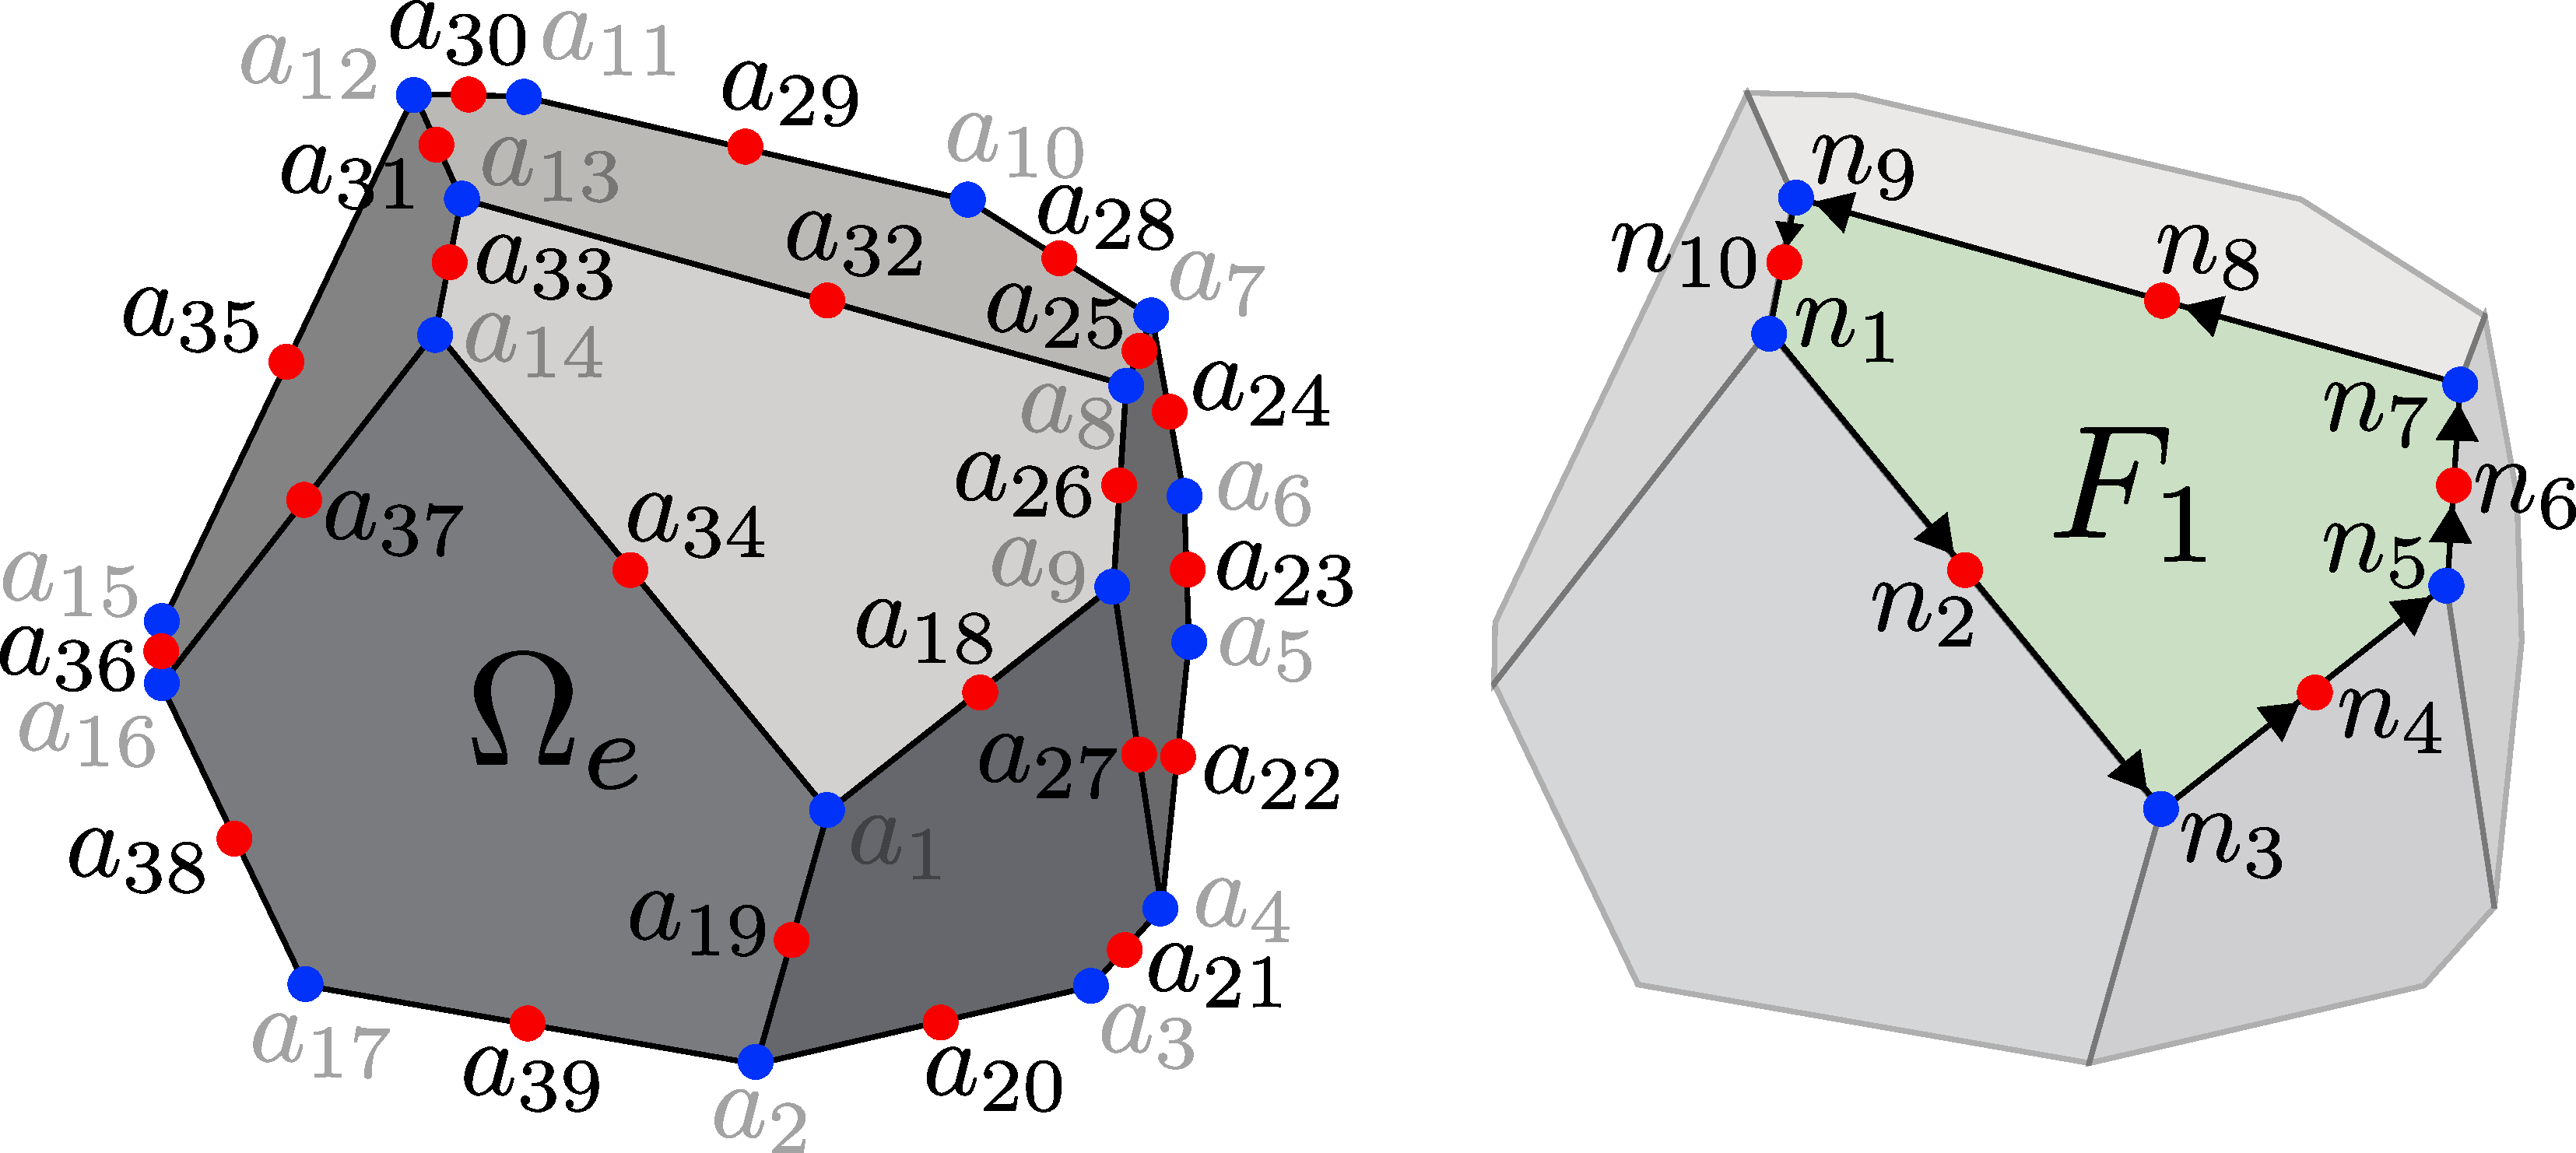
\includegraphics[width = 6.0in]{figures/polyhedron_data_quadratic.pdf}
		\caption{Illustration of the data necessary to describe a quadratic serendipity polyhedral element $\Omega_e$. The local node ID ordering for the face $F_1$ shown would be $\left\{ n_i \right\}_{i=1}^{10} = \left\{ 14, \, 34, \, 1, \, 18, \, 9, \, 26, \, 8, \, 32, \, 13, \, 33 \right\}$.}
		\label{fig:polyhedron_data_quadratic}
	\end{figure}
	
\subsection*{Finite Element Data for Arbitrary Polytopes}

	Traditional Lagrangian finite element methods require each element $\Omega_e \subset \mathcal{B}_0$ to carry the following data (at a minimum) for the purposes of evaluating weak form integrals:
	\begin{itemize}
		\item A list of quadrature weights $\left\{ w_q \right\}_{q=1}^{N^{\Omega_e}_{qp}}$ associated with the quadrature points of the element. The sub-index $q$ induces a local \textit{quadrature point ID}.
		\item Evaluations of the element's nodal shape functions $\left\{ \varphi_a (\mathbf{X}_q) \right\}_{q=1}^{N^{\Omega_e}_{qp}} \, \, \forall a = 1, \ldots, N^{\Omega_e}_V$ at each quadrature point location $\mathbf{X}_q$.
		\item Gradients (with respect to the element's reference coordinates $\mathbf{X}$ at $t = 0$) of the element's nodal shape functions $\left\{ \nabla_X \varphi_a (\mathbf{X}_q) \right\}_{q=1}^{N^{\Omega_e}_{qp}} \, \, \forall a = 1, \ldots, N^{\Omega_e}_V$.
		\item (Optionally) if the element relies upon some form of gradient correction scheme (or more generally, if a Petrov-Galerkin method is employed): evaluations and/or gradients of the element's test functions $\left\{ \phi_a (\mathbf{X}_q), \, \nabla_X \phi_a (\mathbf{X}_q) \right\}_{q=1}^{N^{\Omega_e}_{qp}} \, \, \forall a = 1, \ldots, N^{\Omega_e}_V$ must be stored, as well.
	\end{itemize}
	For solid mechanics applications, material state data (e.g. material properties, internal variables, Cauchy stress) would also need to be stored at each quadrature point location.
	
	Similarly, each boundary face $F_b \subset \Gamma^N_0$ must carry:
	\begin{itemize}
		\item A list of quadrature weights $\left\{ w_q \right\}_{q=1}^{N^{F_b}_{qp}}$ for each quadrature point of the face.
		\item Evaluations of the face's nodal shape functions $\left\{ \varphi_a (\mathbf{X}_q) \right\}_{q=1}^{N^{F_b}_{qp}} \, \, \forall a = 1, \ldots, N^{F_b}_V$ at each quadrature point location $\mathbf{X}_q$.
		\item Gradients (with respect to the face's in-plane reference coordinates $\mathbf{X}$ at $t = 0$) of the face's nodal shape functions $\left\{ \nabla_X \varphi_a (\mathbf{X}_q) \right\}_{q=1}^{N^{F_b}_{qp}} \, \, \forall a = 1, \ldots, N^{F_b}_V$.
		\item If a Petrov-Galerkin method is employed: evaluations and/or gradients of the face's test functions $\left\{ \phi_a (\mathbf{X}_q), \, \nabla_X \phi_a (\mathbf{X}_q) \right\}_{q=1}^{N^{F_b}_{qp}} \, \, \forall a = 1, \ldots, N^{F_b}_V$.
		\item Outward unit normals $\left\{ \mathbf{N}_q \right\}_{q=1}^{N^{F_b}_{qp}}$ to the face $F_b$ at each quadrature point.
	\end{itemize}
	
	The data enumerated above must be determined by means of a specified formulation for how the element's (face's) shape functions and quadrature rule should be constructed. Partitioned element methods address precisely this task. Given an abstract representation for the geometry of a given polyhedral element $\Omega$ (as discussed in the previous section), a PEM formulation proceeds in a number of distinct steps:
	\begin{itemize}
		\item[1.)] The element (and its faces, edges) are appropriately partitioned into cells (facets, segments, verticies).
		\item[2a.)] Individual nodal shape functions are constructed along each edge $E$ of the element.
		\item[2b.)] Individual nodal shape functions are constructed on each face $F$ of the element.
		\item[2c.)] Individual nodal shape functions are constructed on the interior of the element $\Omega$.
		\item[3.)] The discrete finite element data (including quadrature point evaluations of the shape functions and their gradients) are computed and stored by the element.
		\item[4.)] Any auxiliary data (regarding the element's partitioned geometry, etc.) is discarded.
	\end{itemize}
	
	Depending on how the chosen PEM is carried out, the above process can ammount to a relatively large computational expense. However, if a total Lagrangian approach is empolyed within the associated finite element analysis, then the above methodology would only need to be carried out once for each element, at the beginning of the simulation (prior to the first time step). Consequently, the cost of constructing element shape functions in this manner is amortized over the duration of the analysis.
	
	The subsequent sections of this chapter are dedicated to a more detailed discussion of the aforementioned steps taken to construct a given element's partition, and its shape functions.
	
\section{Element Partitioning Schemes}

	In order to construct an arbitrary element's shape functions and quadrature rule.

\subsection*{Edge-Based Partitioning for Star-Convex Elements}

	A star-convex shape $\Omega$ is one for which there exists some point $\mathbf{X}^{\Omega}_0 \in \Omega$ such that the line segment connecting any point $\mathbf{X} \in \Omega$ to $\mathbf{X}^{\Omega}_0$ is entirely contained within $\Omega$. If $\Omega \subset \mathbb{R}^3$ refers to a polyhedron which is star-convex, this further implies that each polygonal face $F \subset \partial \Omega$ is also star-convex with respect to some point $\mathbf{X}^{F}_0 \in F$. Any linear edge $E \subset \partial F$ is star-convex with respect to any point $\mathbf{X} \in E$.
	
	A simple and efficient partitioning scheme is described for polyhedral elements $\Omega$ (and their polygonal faces $F_j$) which are star-convex with respect to their vertex-averaged centroids $\bar{\mathbf{X}}^{\Omega}_0$ (or $\bar{\mathbf{X}}^{F_j}_0$), i.e.
	\begin{equation}
		\bar{\mathbf{X}}^{\Omega}_0 = \frac{1}{N^{\Omega}_V} \sum_{i = 1}^{N^{\Omega}_V} \mathbf{X}_{i}, \quad \text{and} \quad \bar{\mathbf{X}}^{F_j}_0 = \frac{1}{N^{F_j}_V} \sum_{i = 1}^{N^{F_j}_V} \mathbf{X}_{i}.
	\end{equation}
	
	For a given polyhedral element $\Omega_e$, the algorithm proceeds in several steps:
	\begin{itemize}
		\item[1.)] Identify all edges of the polyhedron, and subdivide them into linear segements; each segment should join two adjacent nodes of a given edge.
		\item[2.)] For each face, compute its vertex-averaged centroid $\bar{\mathbf{X}}^{F_j}_0$, and subdivide the face into triangular facets which emanate from $\bar{\mathbf{X}}^{F_j}_0$; each facet should share at most two segments (at least one segment) with $\partial F_j$.
		\item[3a.)] Compute the element's vertex-averaged centroid $\bar{\mathbf{X}}^{\Omega}_0$, and subdivide the element into tetrahedra which emanate from $\bar{\mathbf{X}}^{\Omega}_0$; each tetrahedron should share a single facet with $\partial \Omega$.
		\item[3b.)] Lump into cells any tetrahedra which share a segment belonging to an edge of $\Omega$; each cell should consist of exactly two tetrahedra.
	\end{itemize}
	An illustration of this process is depicted in Figure \ref{fig:partitioning_algorithm}. A similar agorithm may be applied to each boundary face $F_b \subset \Gamma^N_0$, entailing only the first two steps. 
	\begin{figure} [!ht]
		\centering
		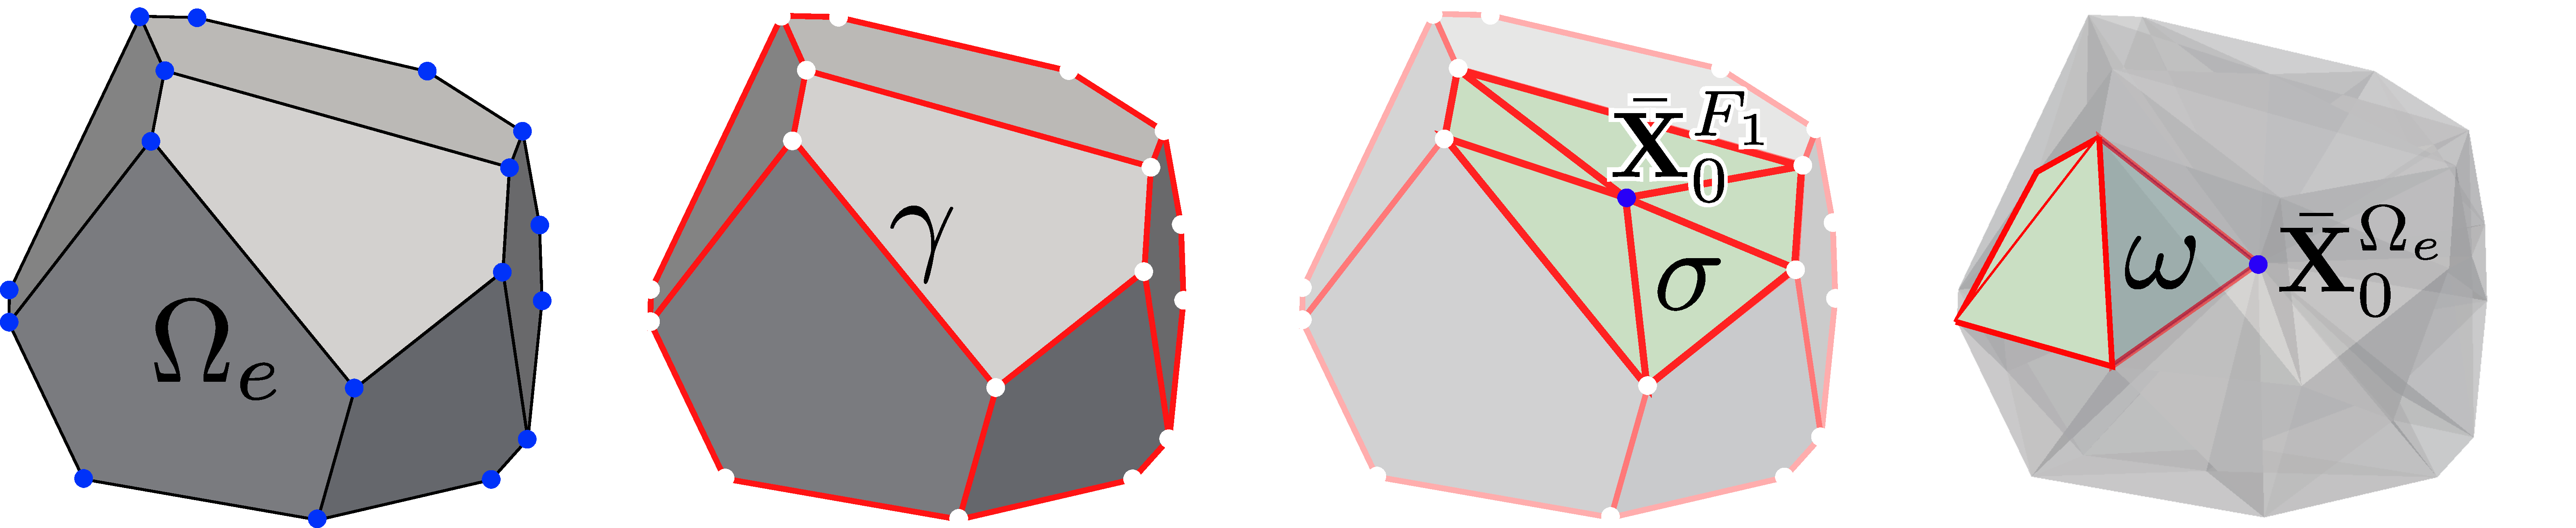
\includegraphics[width = 6.0in]{figures/partitioning_algorithm.pdf}
		\caption{The resulting segment, facet, and cell decomposition for the proposed edge-based partitioning algorithm.}
		\label{fig:partitioning_algorithm}
	\end{figure}
	
	The algorithm can also be naturally extended to accomodate serendipity polyhedral elements with additional nodes belonging to element edges, as depicted in Figure \ref{fig:partitioning_algorithm_quadratic}.
	\begin{figure} [!ht]
		\centering
		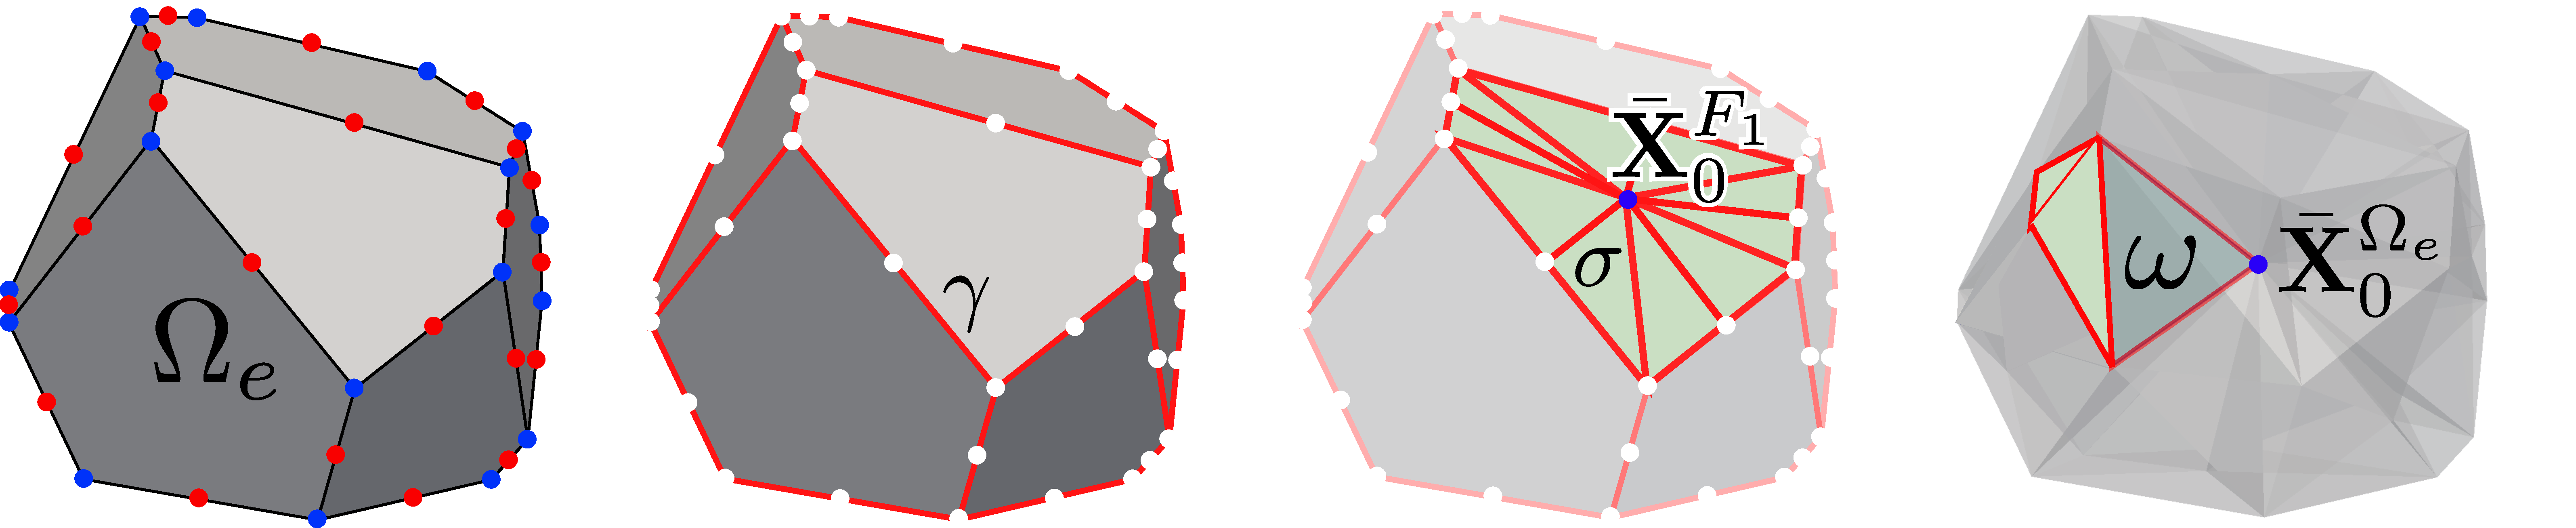
\includegraphics[width = 6.0in]{figures/partitioning_algorithm_quadratic.pdf}
		\caption{The resulting segment, facet, and cell decomposition for the proposed edge-based partitioning algorithm, applied to a quadratic serendipity polyhedral element.}
		\label{fig:partitioning_algorithm_quadratic}
	\end{figure}

\section{Abstract Geometric Data Structures}

	Because partitioned element methods consist of solving a set of 1D, 2D, and 3D problems on each edge, face, and element, there arise a number of similarities between these problems of variable dimension. Namely, the geometric data describing each cell, facet, segment and vertex may be abstracted through the use of generic parent-child (tree-based) data structures. Instead of requiring a separate implementation for the solution of each 1D, 2D, 3D problem, the use of generic programming paradigms are exploited to facilitate a single, unified implementation which is agnostic to the dimensionality of the problem being solved. A number of definitions for the abstract data structures used henceforth are given in the following sections.
	
\subsection*{Geometric Entities}

	\textit{Entities} are defined as the atomic units of the element's geometric partition. An entity may be: a polyhedral cell, a polygonal facet, a linear segment, or a vertex. Entities are defined in terms of their topology -- their relationship to other geometric entities. Specifically, a $3-$dimensional entity (a polyhedral cell $\omega$) is uniquely defined in terms of its $2$-dimensional facets $\sigma \subset \partial \omega$ (termed the ``children'' of $\omega$). Each facet $\sigma$ is in turn considered a $2$-dimensional entity, defined in terms of its $1$-dimensional children (its bounding segements $\gamma \subset \partial \sigma$). An entity of dimension $0$ (a vertex) is identified as having no children.
	
	Each geometric entity may be viewed as a ``node'' in a corresponding tree diagram, as illustrated in Figure \ref{fig:entity_tree}, where the height of a given entity within the tree structure indicates its dimensionality $d$.
	\begin{figure} [!ht]
		\centering
		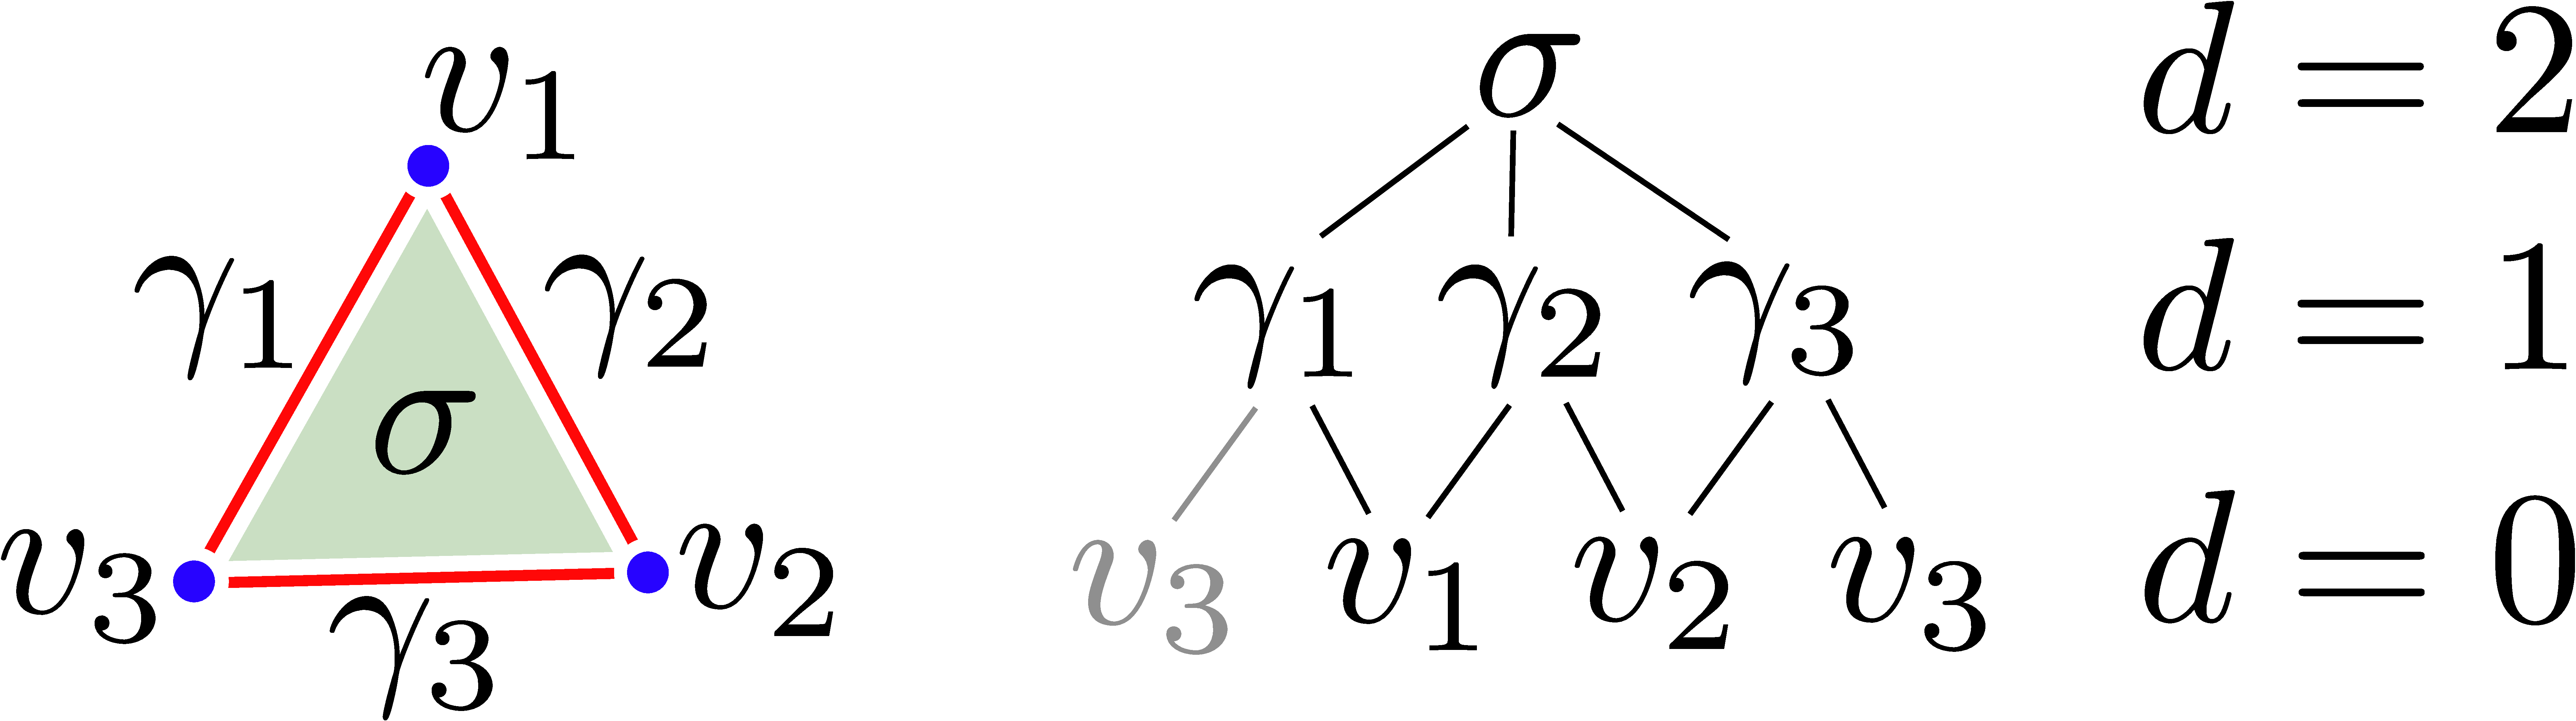
\includegraphics[width = 5.0in]{figures/entity_tree.pdf}
		\caption{A representative entity tree diagram for a $2$-dimensional facet $\sigma$ and its children.}
		\label{fig:entity_tree}
	\end{figure}
	
	Henceforth, we denote by $\varepsilon$ any generic $d-$dimensional entity, and by $\zeta$ any $(d-1)$-dimensional child of $\varepsilon$ (such that $\zeta \subset \partial \varepsilon$). The data stored on a given entity $\varepsilon$ consists of:
	\begin{itemize}
		\item Information (pointers or IDs) refering to the $(d-1)$-dimensional children of $\varepsilon$, and/or information (pointers or IDs) refering to the $(d+1)$-dimensional parents of $\varepsilon$.
		\item An optional orientation/unit direction $\mathbf{N}_\varepsilon$.
		\item A quadrature rule $\left\{ \mathbf{X}_q, w_q \right\}_{q=1}^{N^{\varepsilon}_{qp}}$ defined on $\varepsilon$, or pre-computed monomial integrals $\int_{\varepsilon} \mathbf{X}^\alpha \, d \varepsilon$ for all $|\alpha| \leq k$ (alternatively, the shifted monomial moments $\int_{\varepsilon} (\mathbf{X}-\mathbf{X}_{\varepsilon})^\alpha \, d \varepsilon$ may be stored, instead.)
		\item A list of the basis function IDs which are associated with $\varepsilon$.
	\end{itemize}
	
	The advantage of defining entities in this fashion is that it affords greater flexibility in solving the DG-PEM problem (\ref{eq:dg_poisson}) on elements with arbitrary dimensionality.
	
\subsection*{Sub-Elements}

	Herein, a \textit{sub-element} (generically denoted as $\mathcal{E}$) is defined as a $d-$dimensional polytope (a polyhedral element, a polygonal face, a linear edge, or a node) upon which nodal shape functions are locally constructed and defined. Sub-elements consist of a partition $\mathcal{T}_{\varepsilon} (\mathcal{E})$ of $\mathcal{E}$ into $d-$dimensional entities $\varepsilon$. The boundary of each sub-element $\mathcal{E}$ is comprised of $(d-1)-$dimensional sub-elements, denoted $e \subset \partial \mathcal{E}$ (termed the ``children'' of $\mathcal{E}$, in analog to the definition for geometric entities). A sub-element of dimension $0$ (a node) refers to a single vertex, and possesses no children.
	
	As a representative example, consider the face $F \subset \partial \Omega$ shown in Figure \ref{fig:sub_element}, which is classified as a $2-$dimensional sub-element, whose partition $\mathcal{T}_\sigma (F)$ consists of $2-$dimensional facets $\sigma \subset F$. The boundary/children of $F$ are comprised of $1-$dimensional sub-elements (edges $E \subset \partial F$); in turn, the children of each edge $E$ are the nodes of the element. As with geometric entities, the parent-child relationships between different sub-elements induces a tree-like data stucture, where the height of a given sub-element within the tree corresponds to its dimensionality $d$.
	\begin{figure} [!ht]
		\centering
		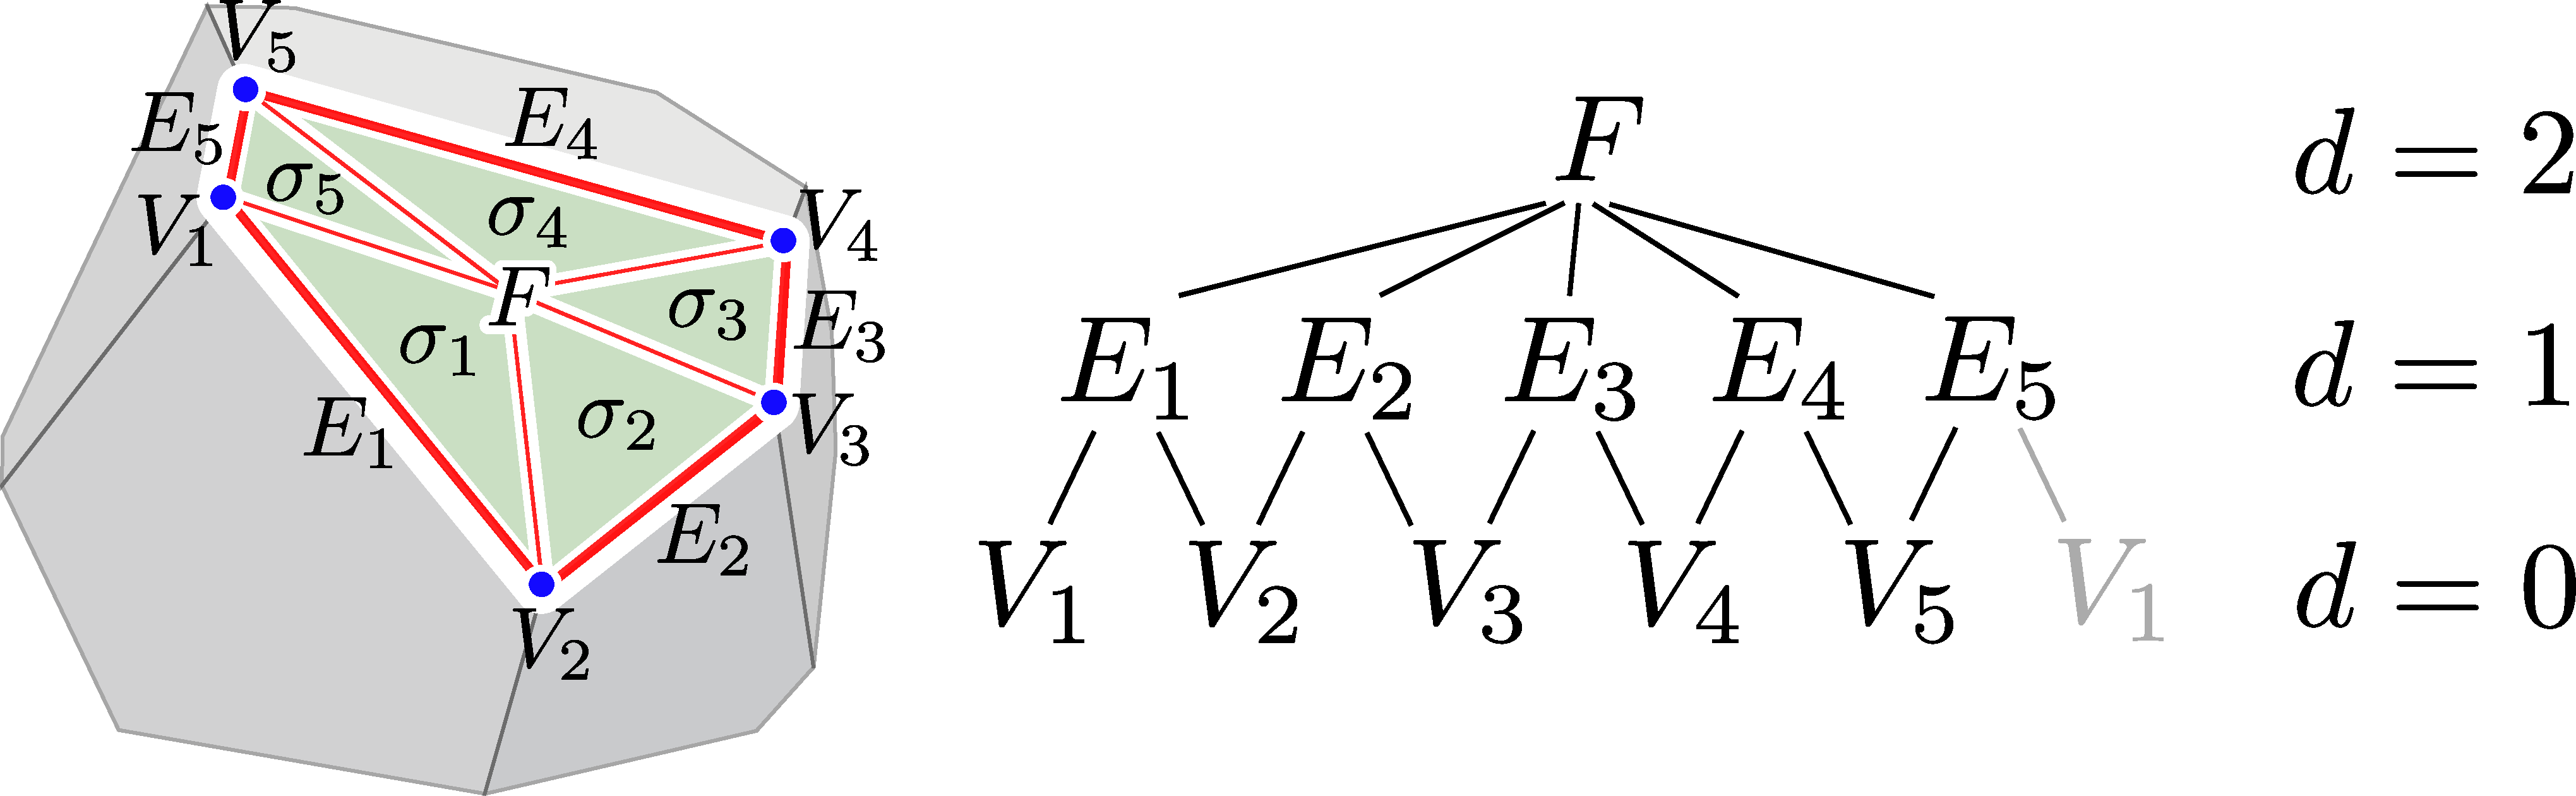
\includegraphics[width = 6.0in]{figures/sub_element.pdf}
		\caption{A representative sub-element tree diagram for a $2$-dimensional face $F$ and its children.}
		\label{fig:sub_element}
	\end{figure}
	
	The data stored for a given sub-element $\mathcal{E}$ consists of:
	\begin{itemize}
		\item Information (pointers or IDs) refering to the $(d-1)$-dimensional entities $\varepsilon \in \mathcal{T}_\varepsilon (\mathcal{E})$ belonging to the partition of $\mathcal{E}$.
		\item Information (pointers or IDs) refering to the $(d-1)$-dimensional children of $\mathcal{E}$ (the sub-elements $e \subset \partial \mathcal{E}$ which constitute the boundary of $\mathcal{E}$).
		\item A list of the basis function IDs which are associated with all entities $\varepsilon \in \mathcal{T}_\varepsilon (\mathcal{E})$.
	\end{itemize}
	
\section{Partition-Based Approximation Spaces}

		As discussed in chapter \ref{ch:pem}, partitioned element methods consider a weak formulation of a given PDE (e.g. Laplace's equation), whose solution is approximated through the specification of a finite dimensional function space $\mathcal{U}^h (\mathcal{E})$ defined on the partition $\mathcal{T}_{\varepsilon} (\mathcal{E})$ of a given sub-element $\mathcal{E}$. The (sub-)element's shape functions are selected as the ``best approximations'' to (harmonic) functions which are contained within the chosen approximation space $\mathcal{U}^h (\mathcal{E})$.
		
		Herein, we consider $\mathcal{U}^h (\mathcal{E})$ to be spanned by a set of basis functions $\left\{ \psi_A \right\}_{A=1}^{N_{bf}}$, such that each basis function $\psi \in \mathcal{U}^h (\mathcal{E})$ is compactly supported over a given geometric entity $\varepsilon \in \mathcal{T}_\varepsilon (\mathcal{E})$ (or patch of entities).
		
		Any function $\varphi^h \in \mathcal{U}^h (\mathcal{E})$ may be written as a linear combination of the basis functions which span $\mathcal{U}^h (\mathcal{E})$, i.e.
		\begin{equation}
			\varphi^h (\mathbf{X}) = \sum_{A=1}^{N_{bf}} \psi_A (\mathbf{X}) \, \varphi_A.
		\end{equation}
		The restriction of $\varphi^h$ to a given geometric entity $\varepsilon$ may be written in terms of only those basis functions $\left\{ \psi^\varepsilon_a \right\}_{a=1}^{N^\varepsilon_{bf}}$ which possess compact support over $\varepsilon$, such that
		\begin{equation}
			\varphi^h|_\varepsilon (\mathbf{X}) = \sum_{a=1}^{N^\varepsilon_{bf}} \psi^\varepsilon_a (\mathbf{X}) \, \varphi_a.
		\end{equation}
		
		To guarantee $P^k (\mathcal{E}) \subset \mathcal{U}^h (\mathcal{E})$ for some desired degree of polynomial completeness $k$, it is necessary for a given entity's local basis $\left\{ \psi^\varepsilon_a \right\}_{a=1}^{N^\varepsilon_{bf}}$ to span $P^k (\varepsilon)$. Arguably the simplest such basis consists of the monomials through order $k$ defined on each entity $\varepsilon \in \mathcal{T}_\varepsilon (\mathcal{E})$. However, the use of monomial bases can lead to ill-conditioning of the DG-PEM problem, particularly as the maximal polynomial degree $k$ is increased. For this reason, other (well-scaled) polynomial bases are reccomended (e.g. the Lagrange polynomials).
		
		Regardless of the chosen basis, each basis function $\psi (\mathbf{X})$ may be expressed as a low-order polynomial (of maximal degree $k$), and can be represented as a linear combination of (possibly shifted) monomials:
		\begin{equation}
			\psi (\mathbf{X}) = \sum_{|\alpha| \leq k} c_\alpha (\mathbf{X}-\mathbf{X}_0)^{\alpha},
		\end{equation}
		where $\alpha = \alpha_1, \ldots, \alpha_d$ is a multi-index, such that $|\alpha| = \alpha_1 + \ldots + \alpha_2$ and $\mathbf{X}^\alpha = X_1^{\alpha_1} \cdots X_d^{\alpha_d}$. Consequently, a given basis function is uniquely defined in terms of its shifted coordinate $\mathbf{X}_0$, and its monomial coefficients $c_\alpha$. The gradient of a given basis function $\nabla \psi (\mathbf{X})$ may in turn be computed via
		\begin{equation}
			\frac{\partial \psi (\mathbf{X})}{\partial X_i} = \sum_{|\alpha| \leq k} \alpha_i c_\alpha (\mathbf{X}-\mathbf{X}_0)^{\alpha_1, \ldots, (\alpha_i - 1), \ldots, \alpha_d}.
		\end{equation}
		
\section{Linearization and Assembly of the \\ DG-PEM Systems of Equations}

	The DG-PEM problem of (\ref{eq:dg_poisson}) may be written as a linear system of equations arising from the chosen basis $\left\{ \psi_A \right\}_{A=1}^{N^\mathcal{E}_{bf}}$ for $\mathcal{U}^h (\mathcal{E})$, such that the basis function coefficients $\varphi_A \, \, \forall A = 1, \ldots, N^\mathcal{E}_{bf}$ representing a given shape function $\varphi^h (\mathbf{X}) = \sum_{A=1}^{N^\mathcal{E}_{bf}} \psi_A (\mathbf{X}) \, \varphi_A$ may be determined as the solution to:
	\begin{equation}
		\sum_{A=1}^{N^\mathcal{E}_{bf}} J_{AB} \, \varphi_A = F_B \quad \forall B = 1, \ldots, N^\mathcal{E}_{bf},
		\label{eq:linearization_dgpem}
	\end{equation}
	where $J_{AB}$ and $F_B$ are computed via an entity-wise assembly process (akin to the methodology employed for assembling finite element systems of equations). However, in addition to assembling local contributions $J^\varepsilon_{ab}$ and $F^\varepsilon_b$ from all $d$-dimensional entities $\varepsilon \in \mathcal{T}_\varepsilon (\mathcal{E})$, here it is also necessary to assemble appropriate contributions from all $(d-1)$-dimensional interfaces $\zeta \in \Gamma_\varepsilon \cup \partial \mathcal{E}$, as well.

	Specifically, each $d$-dimensional entity $\varepsilon \in \mathcal{T}_\varepsilon (\mathcal{E})$ contributes the following local arrays:
	\begin{equation}
			J^{\varepsilon}_{ab} = \int_{\varepsilon} \nabla \psi_a^{\varepsilon} \, \cdot \nabla \psi_b^{\varepsilon} \, d \varepsilon, \quad \forall a, \, b = 1, \ldots, N^{\varepsilon}_{bf},
	\end{equation}
	\begin{equation}
			F^{\varepsilon}_b = \int_{\varepsilon} f_{\mathcal{E}} \, \psi_b^{\varepsilon} \, d \varepsilon \quad \forall b = 1, \ldots, N^{\varepsilon}_{bf},
	\end{equation}
	each $\zeta \in \partial \mathcal{E}$ (which borders a single $d$-dimensional entity $\varepsilon$) contributes:
	\begin{equation}
			J^{\varepsilon}_{ab} = - \int_{\zeta} \bigg( \mathbf{N}_{\zeta} \cdot \nabla \psi^{\varepsilon}_a \, \psi^{\varepsilon}_b + \psi^{\varepsilon}_a \, \nabla \psi^{\varepsilon}_b \cdot \mathbf{N}_{\zeta} \bigg) \, d \zeta + \frac{\alpha_{\zeta0}}{|\zeta|^{\beta_0}} \int_{\zeta} \psi_a^{\varepsilon} \, \psi_b^{\varepsilon} \, d \zeta \quad \forall a, \, b = 1, \ldots, N^{\varepsilon}_{bf},
	\end{equation}
	\begin{equation}
		F^{\varepsilon}_b = - \int_{\zeta} \bar{\varphi} \, \nabla \psi_b^{\varepsilon} \cdot \mathbf{N}_{\zeta} \, d \zeta + \frac{\alpha_{\zeta0}}{|\zeta|^{\beta_0}} \int_{\zeta} \bar{\varphi} \, \psi_b^{\varepsilon} \, d \zeta \quad \forall b = 1, \ldots, N^{\varepsilon}_{bf},
		\label{eq:boundary_term}
	\end{equation}
	and each $\zeta \in \Gamma_\varepsilon$ (which borders two $d$-dimensional entities, $\varepsilon_1$ and $\varepsilon_2$) contributes:
	\begin{align}
			J^{\varepsilon_i \varepsilon_j}_{ab} & = \frac{1}{2} \int_{\zeta} \bigg( (-1)^{j} \mathbf{N}_{\zeta} \cdot \nabla \psi_a^{\varepsilon_i} \, \psi_b^{\varepsilon_j} + (-1)^{i} \psi_a^{\varepsilon_i} \, \nabla \psi_b^{\varepsilon_j} \cdot \mathbf{N}_{\zeta} \bigg) \, d \zeta \\
			& + (-1)^{|i-j|} \frac{\alpha_{\zeta0}}{|\zeta|^{\beta_0}} \int_{\zeta} \psi_a^{\varepsilon_i} \, \psi_b^{\varepsilon_j} \, d \zeta \\
			& + (-1)^{|i-j|} \frac{\alpha_{\zeta1}}{|\zeta|^{\beta_1}} \int_{\zeta} \nabla \psi_a^{\varepsilon_i} \cdot (\mathbf{N}_\zeta \otimes \mathbf{N}_\zeta) \cdot \nabla \psi_b^{\varepsilon_j} \, d \zeta
	\end{align}
	for all $i, \, j = 1, \, 2$, and $a = 1, \ldots, N^{\varepsilon_i}_{bf}$, $b = 1, \ldots, N^{\varepsilon_j}_{bf}$. For the remainder of our discussions, we will consider only the case where $f_\mathcal{E} \equiv 0$ for all sub-elements $\mathcal{E} \subset \Omega$.
	
	For a given $d$-dimensional sub-element $\mathcal{E}$, the assembly of the above terms entails an entity-wise integration of products between basis functions (and their gradients) over $d$-dimensional entities $\varepsilon \in \mathcal{T}_\varepsilon (\mathcal{E})$ and their $(d-1)$-dimensional children $\zeta \in \Gamma_\varepsilon \cup \partial \mathcal{E}$. This may be effected through the use of appropriately defined quadrature rules on each entity, or by pre-computing the monomial integrals over each entity up to some sufficiently high degree (nominally $2k$).
	
	Additionally, it is remarked that the boundary condition $\bar{\varphi}$ is defined independently on every $(d-1)$-dimensional sub-element $e \subset \partial \mathcal{E}$, such that its restriction $\bar{\varphi}|_\zeta$ may be written in terms of the local basis functions $\left\{ \psi^{\zeta}_c \right\}_{c=1}^{N^\zeta_{bf}}$ belonging to a given boundary entity $\zeta \in \partial \mathcal{E}$, i.e.
	\begin{equation}
			\bar{\varphi}|_\zeta (\mathbf{X}) = \sum_{c=1}^{N^\zeta_{bf}} \psi^\zeta_c (\mathbf{X}) \, \bar{\varphi}_c.
	\end{equation}
	For a given $\zeta \in \partial \mathcal{E}$, this yields:
	\begin{equation}
		F^{\varepsilon}_b = \sum_{c=1}^{N^\zeta_{bf}} \bar{J}_{bc} \, \bar{\varphi}_c \quad \forall b = 1, \ldots, N^{\varepsilon}_{bf},
	\end{equation}
	in lieu of (\ref{eq:boundary_term}), where
	\begin{equation}
		\bar{J}_{bc} = - \int_{\zeta} \psi^\zeta_c \, \nabla \psi_b^{\varepsilon} \cdot \mathbf{N}_{\zeta} \, d \zeta + \frac{\alpha_{\zeta0}}{|\zeta|^{\beta_0}} \int_{\zeta} \psi^\zeta_c \, \psi_b^{\varepsilon} \, d \zeta \quad \forall b = 1, \ldots, N^{\varepsilon}_{bf}, \, c = 1, \ldots, N^\zeta_{bf}.
	\end{equation}
	Consequently, we may re-write the right-hand side of (\ref{eq:linearization_dgpem}) as a linear mapping from the basis coefficients $\bar{\varphi}_C$ which determine the boundary function $\bar{\varphi} (\mathbf{X}) = \sum_{C=1}^{N^{\partial \mathcal{E}}_{bf}} \psi_C (\mathbf{X}) \, \bar{\varphi}_C$:
	\begin{equation}
		\sum_{A=1}^{N^{\mathcal{E}}_{bf}} J_{AB} \, \varphi_A = \sum_{C=1}^{N^{\partial \mathcal{E}}_{bf}} \bar{J}_{BC} \, \bar{\varphi}_C \quad \forall B = 1, \ldots, N^{\mathcal{E}}_{bf},
	\end{equation}
	which may alternatively be written in matrix-vector format:
	\begin{equation}
		\mathbf{J} \, \boldsymbol{\varphi} = \bar{\mathbf{J}} \, \bar{\boldsymbol{\varphi}}.
	\end{equation}
	
	The above system of equations can be solved to obtain a linear mapping from $\bar{\boldsymbol{\varphi}}$ to $\boldsymbol{\varphi}$, denoted $\mathbf{M} = \mathbf{J}^{-1} \bar{\mathbf{J}} : \mathbb{R}^{N^{\partial \mathcal{E}}_{bf}} \mapsto \mathbb{R}^{N^{\mathcal{E}}_{bf}}$. This mapping may be utilized to define the shape functions in a recursive fashion (over the children of each sub-element, in succession), ultimately yielding a representation for the shape functions on $\mathcal{E}$ in terms of only nodal evaluations $\varphi|_{V}$. This process is discussed in greater detail in the following section.
	
\section{Hierarchial Construction of Shape Functions}

	For a given polyhedral element $\Omega \subset \mathbb{R}^d$, we presume that each shape function $\varphi_A$ is associated with a particular node $V_A$ of the element, such that
	\begin{equation}
		\varphi_A |_{V_B} = \delta_{AB} \quad \forall A, \, B = 1, \ldots, N_V.
	\end{equation}
	
	Additionally, for the sake of simplicity and computational efficiency, it is suggested that the shape functions along each linear edge $E$ be constructed from the Lagrange polynomials which interpolate the nodal values of that edge, i.e.
	\begin{equation}
		\varphi_A |_{E} (\mathbf{X}) = \sum_{b = 1}^{N^E_V} \psi_b (\mathbf{X}) \, \varphi_A |_{V_b}.
	\end{equation}

\section{Construction of Quadrature Rules}



\section{Numerical Conditioning of the \\ DG-PEM Systems of Equations}

As a representative example, let us consider a given polygonal PEM element $\Omega \subset \mathbb{R}^2$. The element is subdivided into polygonal cells $\sigma_c$, linear segments $\gamma_b$ which bound each cell, and verticies $v_a$ which bound each segment. Additionally, the element itself is bounded by edges $E_I$ comprising subsets of segments $\gamma_{Ib}$, and each edge is bounded by nodes $N_A$ collocated with the geometric verticies of the element, which bear the primary degrees of freedom $u_A$ of the element (an edge may also contain a number of ``internal'' nodes, as well.) The element's ``partition'' $\mathcal{T}$ is defined as the union of all cells, segments, and verticies. An arbitrary subset $\omega \in \mathcal{T}$ refers generically to an individual vertex, segment, or cell.

The goal of the PEM is to construct suitable representations of the nodal shape functions $\varphi_A (\mathbf{x}) \, \forall \mathbf{x} \in \Omega$ defined in a piece-wise fashion on the partition of the element. The space of functions under consideration $\mathcal{U}_k (\Omega)$ corresponds to a broken Sobolev space, defined as
\begin{equation}
        \mathcal{U}_k (\Omega) := \left\{ u \in L^2 (\Omega) \, : \, u |_{\omega} \in P_k (\omega) \, \forall \omega \in \mathcal{T} \right\},
\end{equation}
where $u|_\omega$ denotes the restriction of $u$ to $\omega \subset \Omega$, and where $P_k (\omega)$ denotes the space of polynomials on $\omega$ of maximal degree $k$. Classical approaches have sought to represent a given nodal shape function as a (discontinuous) piece-wise linear function over the element (i.e. $\varphi_A \in \mathcal{U}_1 (\Omega)$), such that
\begin{equation}
     \varphi_A |_\omega (\mathbf{x}) = c_{\omega} + \mathbf{g}_{\omega} \cdot \mathbf{x}.
\end{equation}
Recent investigations have explored the use of higher-order interpolants in an effort to achieve higher-order polynomial completeness, i.e. for an arbitrary $u \in \mathcal{U}_k (\Omega)$, we would have (in multi-index notation)
\begin{equation}
     u |_\omega (\mathbf{x}) = \sum_{|\alpha| \leq k} a_{\omega}^{(\alpha)} \mathbf{x}^{\alpha}.
\end{equation}

The current approach to construct the shape functions of a given element proceeds in a hierarchal fashion (in 2D):
\begin{itemize}
        \item[(1.)] For every edge $E_I$, determine a linear transformation $\mathbf{F}_I : u_A \mapsto u|_{E_I}$ which maps the edge's nodal values $u_A$ to the piece-wise polynomial representation of $u$ on the edge's partition of segments.
        \item[(2.)] Determine a linear transformation $\mathbf{G} : u|_{\partial \Omega} \mapsto u|_{\sigma_c}$ which maps the piece-wise polynomial representation of $u$ on the boundary of the element to its piece-wise representation on the element's partition of cells.
        \item[(3.)] Compose all mappings from (1.) and (2.) to obtain a final linear transformation $\mathbf{M} : u_A \mapsto u|_{\sigma_c}$ which maps the element's nodal values to its piece-wise polynomial representation on the element's cell partition.
\end{itemize}
The individual nodal shape functions are obtained by considering the values of $ u|_{\sigma_c}$ that result from setting a given node's value $u_A = 1$ and all others equal to zero.

For the transformation $\mathbf{G}$, in particular, we should prefer that such a mapping yield a piece-wise representation of $u|_{\sigma_c}$ on the complex of cells which is both relatively ``smooth'' and ``continuous.'' More precisely, we require that any $u|_{\sigma_c}$ obtained through $\mathbf{G}$ be the unique minimizer of a prescribed functional $\mathcal{G}$:
\begin{equation}
        \mathcal{G} := \beta_0 \sum_{b \in \bar{\mathcal{B}}} \frac{1}{2} \int_{\gamma_b} [\![ u ]\!]^2 \, ds + \beta_1 \sum_{b \in \mathcal{B}} \frac{h_b^2}{2} \int_{\gamma_b} [\![ \mathbf{n} \cdot \nabla u ]\!]^2 \, ds
\end{equation}
which represents a weighted measure of compatibility and smoothness in the piece-wise representation of $u$ over the element's cell partition. If we choose to represent each $u|_{\sigma_c}$ using a monomial basis, i.e.
\begin{equation}
     u |_{\sigma_c} (\mathbf{x}) = \sum_{|\alpha| \leq k} a_{\sigma_c}^{(\alpha)} \mathbf{x}^{\alpha} = \mathbf{m} \cdot \mathbf{a}_{\sigma_c}
\end{equation}
where $\mathbf{m}$ is a vector of monomials and $\mathbf{a}_{\sigma_c}$ is a vector of the corresponding (unknown) monomial coefficients for a given cell $\sigma_c$, then we may formulate our minimum problem as
\begin{equation}
        \min_{\mathbf{a}_{\sigma_c}} \mathcal{G} (\mathbf{a}_{\sigma_c}),
\end{equation}
and the unique minimizer of $\mathcal{G}$ will satisfy
\begin{equation}
        \frac{\partial \mathcal{G}}{\partial \mathbf{a}_{\sigma_c}} = \mathbf{0} \quad \forall c.
\end{equation}

Let us momentarily consider an individual segment $\gamma_b$ which separates two cells, $\sigma_{b1}$ and $\sigma_{b2}$. Note that
\begin{equation}
        \int_{\gamma_b} [\![ u ]\!]^2 \, ds = (\mathbf{a}_{\sigma_{b1}} - \mathbf{a}_{\sigma_{b2}}) \cdot \left[ \int_{\gamma_b} \mathbf{m} \otimes \mathbf{m} \, ds \right] (\mathbf{a}_{\sigma_{b1}} - \mathbf{a}_{\sigma_{b2}}),
\end{equation}
and
\begin{equation}
        h_b^2 \int_{\gamma_b} [\![ \mathbf{n} \cdot \nabla u ]\!]^2 \, ds = (\mathbf{a}_{\sigma_{b1}} - \mathbf{a}_{\sigma_{b2}}) \cdot \left[ h_b^2 \int_{\gamma_b} \frac{\partial \mathbf{m}}{\partial n} \otimes \frac{\partial \mathbf{m}}{\partial n} \, ds \right] (\mathbf{a}_{\sigma_{b1}} - \mathbf{a}_{\sigma_{b2}}),
\end{equation}
where we prescribe $h_b = (|\sigma_{b1}| + |\sigma_{b2}|)/|\gamma_{b}|$ to obtain a proportional scaling of the two integral contributions to $\mathcal{G}$. If we define moment matrices $\mathbf{M}_{0b}$ and $\mathbf{M}_{1b}$ as
\begin{equation}
        \mathbf{M}_{0b} \equiv \int_{\gamma_b} \mathbf{m} \otimes \mathbf{m} \, ds
\end{equation}
\begin{equation}
        \mathbf{M}_{1b} \equiv h_b^2 \int_{\gamma_b} \frac{\partial \mathbf{m}}{\partial n} \otimes \frac{\partial \mathbf{m}}{\partial n} \, ds
\end{equation}
then we may express the local contribution from segment $\gamma_b$ to $\mathcal{G}$ as
\begin{equation}
        \mathcal{G}_b = \frac{1}{2} \left\{ \begin{array}{c} \mathbf{a}_{\sigma_{b1}} \\ \mathbf{a}_{\sigma_{b2}} \end{array} \right\} \cdot \bigg( \beta_0 \left[ \begin{array}{cc} \mathbf{M}_{0b} & - \mathbf{M}_{0b} \\ - \mathbf{M}_{0b} & \mathbf{M}_{0b} \end{array} \right] + \beta_1 \left[ \begin{array}{cc} \mathbf{M}_{1b} & - \mathbf{M}_{1b} \\ - \mathbf{M}_{1b} & \mathbf{M}_{1b} \end{array} \right] \bigg) \left\{ \begin{array}{c} \mathbf{a}_{\sigma_{b1}} \\ \mathbf{a}_{\sigma_{b2}} \end{array} \right\},
\end{equation}
or more concisely:
\begin{equation}
        \mathcal{G}_b = \frac{1}{2} \mathbf{a}_{\sigma_{b_{1,2}}} \cdot \mathbf{J}_b \mathbf{a}_{\sigma_{b_{1,2}}}.
\end{equation}
The matrix $\mathbf{J}_b$ expressed in the above equation constitutes a local contribution from segment $\gamma_b$ to the Jacobian of $\partial \mathcal{G} / \partial \mathbf{a}_{\sigma_c}$ (i.e. to $\mathbf{J} = \partial^2 \mathcal{G} / \partial \mathbf{a}_{\sigma_c} \partial \mathbf{a}_{\sigma_d}$, which will ultimately be inverted when we solve for the unknown monomial coefficients in each cell). Consequently, it becomes of interest to investigate the condition number for the Jacobian of $\partial \mathcal{G} / \partial \mathbf{a}_{\sigma_c}$ in terms of our choice of polynomial basis.

We proceed in obtaining a rough approximation to $\kappa (\mathbf{J})$ by examining a particular element whose partition contains only one cell $\sigma$. For this simple case, we have
\begin{equation}
        \mathbf{J} = \beta_0 \int_{\partial \sigma} \mathbf{m} \otimes \mathbf{m} \, ds = \beta_0 \sum_{\forall b} \mathbf{M}_{0b}.
\end{equation}
Let us approximate the bounds for each monomial integral. By application of the triangle inequality to the Riemann integral of the monomials over $\partial \sigma$, we obtain
\begin{equation}
       \bigg| \int_{\partial \sigma} m_i m_j \, ds \bigg| \leq \int_{\partial \sigma} | m_i m_j | \, ds,
\end{equation}
and by the max-min inequality, we find
\begin{equation}
       \int_{\partial \sigma} | m_i m_j | \, ds \leq \max_{\mathbf{x} \in \partial \sigma} \{ | m_i m_j | \} \int_{\partial \sigma} \, ds.
\end{equation}
Since the monomials are continuous functions on $\partial \sigma$, by the mean-value theorem we have
\begin{equation}
        m^*_i m^*_j \int_{\partial \sigma} \, ds = \int_{\partial \sigma} m_i m_j \, ds
\end{equation}
and by extension
\begin{equation}
        | m^*_i m^*_j | \int_{\partial \sigma} \, ds = \bigg| \int_{\partial \sigma} m_i m_j \, ds \bigg|
\end{equation}
for some $m^*_i m^*_j$ evaluated at a particular $\mathbf{x}^* \in \partial \sigma$. By the extreme value theorem and the continuity of $|m_i m_j|$,
\begin{equation}
         \min_{\mathbf{x} \in \partial \sigma} \{ | m_i m_j | \} \leq | m^*_i m^*_j | \leq \max_{\mathbf{x} \in \partial \sigma} \{ | m_i m_j | \}.
\end{equation}
Therefore,
\begin{equation}
         \min_{\mathbf{x} \in \partial \sigma} \{ | m_i m_j | \} \int_{\partial \sigma} \, ds \leq | m^*_i m^*_j | \int_{\partial \sigma} \, ds = \bigg| \int_{\partial \sigma} m_i m_j \, ds \bigg|,
\end{equation}
and our bounds are thus,
\begin{equation}
       \min_{\mathbf{x} \in \partial \sigma} \{ | m_i m_j | \} \int_{\partial \sigma} \, ds \leq \bigg| \int_{\partial \sigma} m_i m_j \, ds \bigg| \leq \max_{\mathbf{x} \in \partial \sigma} \{ | m_i m_j | \} \int_{\partial \sigma} \, ds.
\end{equation}
These bounds are approximate, and in particular, the lower bound may be equal to zero in some cases. For our analysis of the condition number, these bounds prove to be insufficient. Indeed, the monomials of odd degree may well be equal to zero, but those of even degree are guaranteed to be non-zero for any cell $\sigma$ with finite area. It suffices to consider the projection $\mathcal{P} (\sigma)$ of the domain of $\sigma$ onto any linear subspace of dimension $1$ which yields a characteristic minimum dimension $d_{\min}$:
\begin{equation}
	d_{\min} = \inf_{\mathcal{P} (\sigma)} \{ \sup_{x, y \in \mathcal{P} (\sigma)} \{ | x - y | \} \}.
\end{equation}
Intuitively, $d_{\min}$ is the smallest possible dimension of any bounding box which contains $\sigma$. It is not difficult to see that the integral of any monomial of even degree $2p$ will be bounded from below by a finite term of order $O(d_{\min}^{2p})$. This remark will find significance later on.

Returning to the Jacobian $\mathbf{J}$, its entries $J_{ij}$ correspond to
\begin{equation}
        J_{ij} = \beta_0 \int_{\partial \sigma} m_i m_j \, ds.
\end{equation}
By Gershgorin's theorem, we may determine approximate bounds for every eigenvalue $\lambda$ of $\mathbf{J}$, such that
\begin{equation}
        | \lambda - J_{ii} | \leq \sum_{j \neq i} | J_{ij} | \quad \forall i,
\end{equation}
and consequently
\begin{equation}
        c_i - d_i \leq \lambda \leq c_i + d_i \quad \forall i,
\end{equation}
where
\begin{equation}
        c_i = \beta_0 \int_{\partial \sigma} m_i m_i \, ds,
\end{equation}
\begin{equation}
        d_i = \sum_{j \neq i} \bigg| \beta_0 \int_{\partial \sigma} m_i m_j \, ds \bigg|.
\end{equation}
The condition number of $\mathbf{J}$ is then bounded by
\begin{equation}
        \kappa (\mathbf{J}) \leq \frac{\max_i \{ | c_i + d_i | \}}{\min_i \{ | c_i - d_i | \}}.
\end{equation}
By the triangle inequality
\begin{equation}
        | c_i + d_i | \leq | c_i | + | d_i | = \sum_{j} \bigg| \beta_0 \int_{\partial \sigma} m_i m_j \, ds \bigg|,
\end{equation}
such that
\begin{equation}
        \kappa (\mathbf{J}) \leq \frac{\max_i \{ | c_i + d_i | \}}{\min_i \{ | c_i - d_i | \}} \leq \frac{\max_i \{ | c_i | + | d_i | \}}{\min_i \{ | c_i - d_i |  \}}.
\end{equation}
where
\begin{equation}
        \max_i \{ | c_i | + | d_i | \} = \max_i \left\{ \sum_{j} \bigg| \beta_0 \int_{\partial \sigma} m_i m_j \, ds \bigg| \right\}.
\end{equation}
Provided $\beta_0 > 0$,
\begin{equation}
        \max_i \{ | c_i | + | d_i | \} \leq \beta_0 \max_i \left\{ \sum_{j} \max_{\mathbf{x} \in \partial \sigma} \{ | m_i m_j | \} \right\} \int_{\partial \sigma} \, ds.
\end{equation}
Since $\mathbf{J}$ is assumed to be positive definite, $c_i > 0$ and $c_i - | d_i | > 0$, and we may write (approximately)
\begin{equation}
        \min_i \{ | c_i  - d_i | \} \approx \min_i \{ | c_i | \} \geq \beta_0 \min_i \left\{ \beta_0 \int_{\partial \sigma} m_i m_i \, ds \right\}.
\end{equation}

Suppose there exist some maximum and minimum radii $r_{\max}$ and $r_{\min}$ such that $r_{\min} \leq || \mathbf{x} ||_2 \leq r_{\max} \, \forall \mathbf{x} \in \partial \sigma$ and  $r_{\max} > r_{\min} \geq 0$. Note that if $r_{\max} > 1$, then
\begin{equation}
        \max_i \left\{ \sum_{j} \max_{\mathbf{x} \in \partial \sigma} \{ | m_i m_j | \} \right\} = O (r_{\max}^{2k}),
\end{equation}
and if $r_{\max} < 1$, then
\begin{equation}
        \max_i \left\{ \sum_{j} \max_{\mathbf{x} \in \partial \sigma} \{ | m_i m_j | \} \right\} = O (1).
\end{equation}
Separately, if $r_{\min} > 1$, then
\begin{equation}
        \min_i \left\{ \int_{\partial \sigma} m_i m_i \, ds \right\} \geq \min_i \left\{ \min_{\mathbf{x} \in \partial \sigma} \{ | m_i m_i | \} \right\} \int_{\partial \sigma} \, ds = O (1),
\end{equation}
and if $r_{\min} < 1$, then
\begin{equation}
         \min_i \left\{ \int_{\partial \sigma} m_i m_i \, ds \right\} \geq \min_i \left\{ \min_{\mathbf{x} \in \partial \sigma} \{ | m_i m_i | \} \right\} \int_{\partial \sigma} \, ds = O (r_{\min}^{-2k}).
\end{equation}
If $r_{\min} = 0$ (or when $d_{\min} > 2r_{\min}$), we invoke our alternative lower bound for the monomial integrals of even degree, such that
\begin{equation}
         \min_i \left\{ \int_{\partial \sigma} m_i m_i \, ds \right\} = O (d_{\min}^{-2k}).
\end{equation}
Now, define a characteristic dimension $h$ satisfying
\begin{equation}
        h = \frac{\max \{ r_{\max}, \, 1 \}}{\min \{ \max \{d_{\min}/2, \, r_{\min} \}, \, 1 \}}.
\end{equation}
The approximate condition number of $\mathbf{J}$ for a given cell $\sigma$ with characteristic dimension $h$ using a monomial basis up to order $k$ is then
\begin{equation}
        \kappa (\mathbf{J}) \approx O(h^{2k}).
	\label{eq:estimate}
\end{equation}

Following a number of numerical experiments, it was determined that the estimate in (\ref{eq:estimate}) is quite accurate, and illuminates a number of key points:
\begin{itemize}
	\item[(I.)] The condition number depends upon the dimensions of the element, and more specifically, upon the dimensions of its partition.
	\begin{itemize}
		\item[a.] Isotropically scaling an element will change the condition number of the resulting PEM linear systems, for better or for worse. This would seem to justify the idea of rescaling PEM elements into a corresponding ``parent'' domain -- ideally one which minimizes $h$. Shape functions and gradients would then be computed in the parent configuration, and subsequently mapped back into the element's physical configuration.
		\item[b.] Choosing the element's reference coordinate system poorly may subtly impact the conditioning of the PEM linear systems. This further justifies the idea that the element's local coordinate system should be shifted in such a way as to minimize $h$. However, certain choices of reference coordinate may be preferable/optimal for the different tope-level minimum problems. Namely, recent numerical experiments have revealed that the solution inaccuracies caused by nearly planar faces can be effectively mitigated when the element's reference coordinate is chosen to lie on or near the warped face(s). This finding may warrant the reconsideration of a local coordinate system being used for every cell (or at the very least, for every tope) of the element.
		\item[c.] Elements with unequal dimensions (i.e. thin elements) will unavoidably suffer from issues of poor conditioning due to a larger relative value of $h$ (regardless of isotropic scaling). The natural temptation would be to scale the element anisotropically in an effort to achieve better conditioning. However, this would need to be done with care; every tope of the element would need to be scaled independently, according to a given tope's dimensions alone. This condition is necessary to guarantee inter-face compatibility between elements, as two anisotropically scaled elements would not, in general, produce identical shape functions on their shared face.
	\end{itemize}
	\item[(II.)] The condition number becomes drastically worse when higher order monomials are used.
	\begin{itemize}
		\item[a.] This explains a great deal about why the quadratic PEM elements have performed so poorly in convergence studies up to this point: not only does $h$ become worse under mesh refinement, but the condition number scales as $O(h^4)$ for quadratic elements, leading to significant inaccuracies in the shape function computations, and subsequent losses in solution accuracy.
		\item[b.] Unfortunately, this makes thin quadratic elements even more sensitive to the relative scaling of $h$. It is unclear whether or not anisotropically rescaling the elements will sufficiently improve matters.
	\end{itemize}
	\item[(III.)] Perhaps most importantly: the strong dependence of the condition number upon $h$ and $k$ is largely a consequence of our specific choice of polynomial basis (i.e. the monomial basis).
	\begin{itemize}
		\item[a.] Because the solution unknowns that we seek are monomial coefficients, it is to be expected that the constant, gradient (and curvature) coefficients may differ by orders of magnitude, depending on the relative scale of the element in physical space.
		\item[b.] A more robust solution to the aforementioned issues of conditioning might be obtained through the selection of a different polynomial basis for $P_k (\Omega)$ (other than the monomial basis). In particular, the use of an orthonormal polynomial basis (with respect to an appropriately defined norm on an arbitrary element domain) could entirely circumvent the problem of poor conditioning. To prove this, we would need to illustrate that the resulting condition number of $\mathbf{J}$ using an orthonormal polynomial basis is less sensitive to both $h$ and $k$.
	\end{itemize}
\end{itemize}

\subsection{The Effect of Element Scaling}
\subsection{On the Choice of an Appropriate PEM Basis}
